\section{Imagenette, a Vision Transformer, and Feature Visualization}
\label{sec:feature-visualization}
Small CIFAR images cannot show the visual detail needed to investigate
many feature hypotheses. We therefore add higher-resolution photographs,
a vision transformer, and optimized and controlled stimuli. The aim is
to triangulate a coordinate's behavior using several kinds of evidence,
as advocated in~\cite{olah2020zoom,olah2017featureVis}. Similar-looking
visualizations alone do not establish that our coordinates implement the
InceptionV1 features or circuits studied in those works.

\subsection{Datasets, backbones, and surrogate training}
\label{sub:imagenette-protocol}
Imagenette contains ten ImageNet categories, including English springers,
churches, and vehicles. Imagewoof contains ten dog-breed categories
\cite{howardImagenette}. We use the official 320-pixel archives. Within
each Imagenette class, sort archive member paths lexicographically and
take the first 25 training photographs and first ten validation
photographs. The first 20 training photographs fit the surrogate, and
five are reserved for calibration. This gives 200 training, 50
calibration, and 100 test images. A further 100 images, the first ten
validation photographs per Imagewoof class, form a transfer collection.
Imagewoof images do not train the surrogate or select its coordinates.
These deterministic subsets support inspectable examples rather than
population-level performance claims.

Convert images to RGB, resize the shorter edge to 256 pixels with bicubic
interpolation, and take a central $224\times224$ crop. Normalize channels
by the ImageNet mean and standard deviation before the backbone. Save
both original JPEG bytes and the cropped pixels, with archive-member
identifiers and content hashes. Because Imagenette is an ImageNet subset,
the ResNet backbone may have seen these images during pretraining. A
held-out surrogate split is not evidence of an unseen backbone dataset;
we do not assert a pretraining-overlap exclusion for DINOv2 either.

We compare the frozen ResNet34 with a frozen DINOv2 ViT-S/14
\cite{dosovitskiy2021vit,oquab2024dinov2}. The ResNet representation is the
same complete third residual stage used previously, now with a
$14\times14$ grid of 256-dimensional sites. The DINOv2 representation is
the final layer-normalized output of its twelve transformer blocks:
a $16\times16$ grid of 384-dimensional patch tokens. The leading CLS
token is excluded, and this checkpoint has no register tokens. The exact
Hugging Face checkpoint revision and its hashes are released. A patch's
position identifies a token, not a local receptive field: global
self-attention can transmit evidence from anywhere in the crop.

For each backbone separately, subtract the training-site channel mean
and divide by the training-site standard deviation, floored at
$10^{-6}$. Train a nonnegative Top-32 SAE with twice the backbone width:
512 coordinates for ResNet and 768 for DINOv2. Initialize encoder weights
from the transpose of the unit-column decoder and set both biases to
zero. Train for 30 epochs with Adam, learning rate 0.001, batch size 512,
and seed 2027; normalize decoder columns after every update. Centering
permits signed dense inputs while the sparse codes remain nonnegative,
as required by the context construction. Reconstruction statistics are
computed after restoring the original channel units.

\begin{table}[tbp]
\centering
\begin{tabular}{lrrr}
\toprule
Model & Test $R^{2}_{\mathrm{tr}}$ & Transfer $R^{2}_{\mathrm{tr}}$ & Active \\
\midrule
ResNet34 & 0.878 & 0.881 & 512/512 \\
DINOv2 & 0.707 & 0.596 & 768/768 \\
\bottomrule
\end{tabular}
\caption{Reconstruction in original channel units and active training
coordinates. Test denotes Imagenette; transfer denotes Imagewoof. All models
use the training mean as the reconstruction baseline.}
\label{tab:imagenette-metrics}
\end{table}

Imagenette test reconstruction is 0.878 for ResNet and 0.707 for DINOv2;
Imagewoof transfer reconstruction is 0.881 and 0.596, respectively.
Every dictionary coordinate is active somewhere on the training sites.
The DINOv2 transfer drop limits the fidelity of its sparse representation
on the dog-breed collection, even when individual galleries look coherent.
The reserved calibration images are not used to optimize a threshold or
choose a checkpoint. Fixed training settings and the final epoch are
used throughout. The two backbones also differ in pretraining, width,
site count, and surrogate dictionary size; this is a matched protocol,
not a controlled claim that architecture alone explains a difference.

\subsection{Photographs and optimized feature stimuli}
\label{sub:optimized-features}
For each backbone, select distinct coordinates for English springer and
church by the training contrast in~\cref{eq:feature-contrast}. Rank all
100 Imagenette test images for each selected coordinate, retaining
mismatched labels. Apply the springer-selected coordinate unchanged to
all 100 Imagewoof images. Coordinates are selected independently across
backbones; matching class-selection criteria do not align dictionary
indices or prove equivalent feature meanings.

\begin{figure}[p]
    \centering
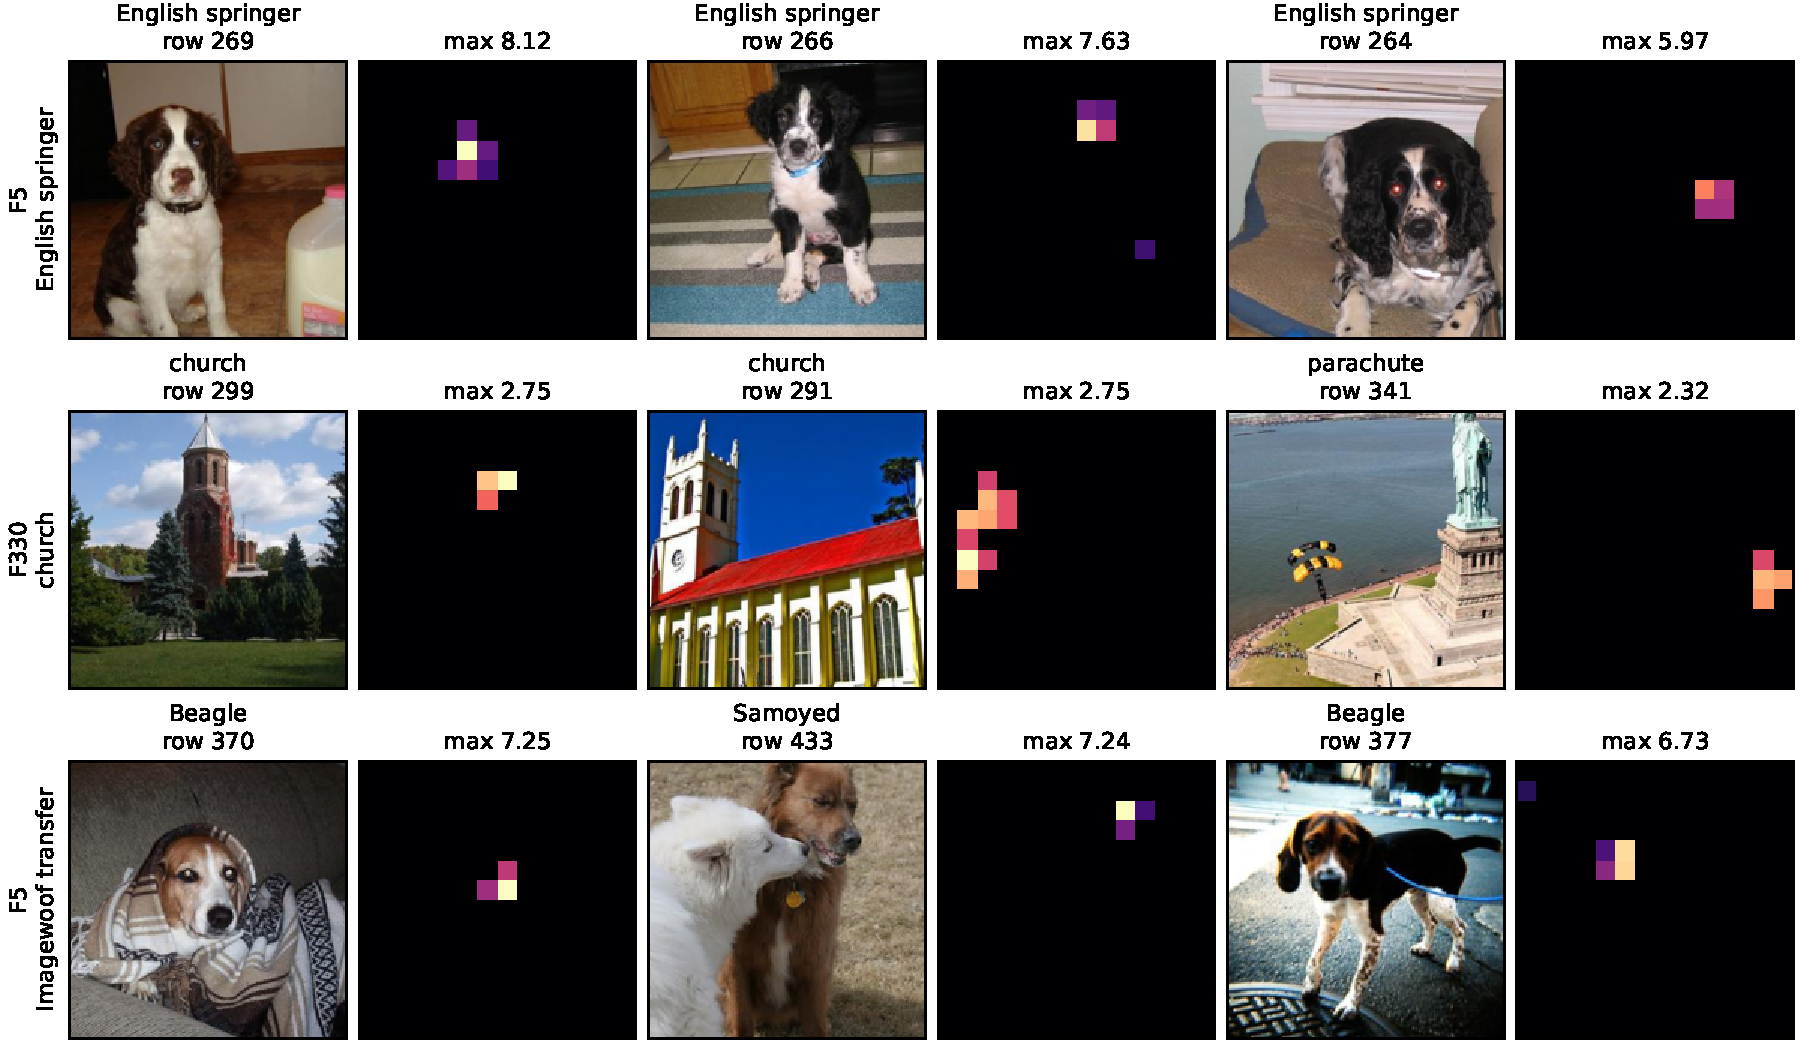
\includegraphics[width=\linewidth]{figures/imagenette_resnet34_codexgen.pdf}
    \caption{ResNet34 sparse coordinates on Imagenette and Imagewoof.
        The first two rows show the strongest Imagenette test responses for
        training-selected springer and church coordinates. The last row applies
        the springer coordinate to Imagewoof without retraining. Each
        photograph
        is followed by its site-code map, with a common color scale within the
        row. Actual labels, stored dataset rows, and maxima are displayed.}
    \label{fig:imagenette-resnet}
\end{figure}

\begin{figure}[p]
    \centering
    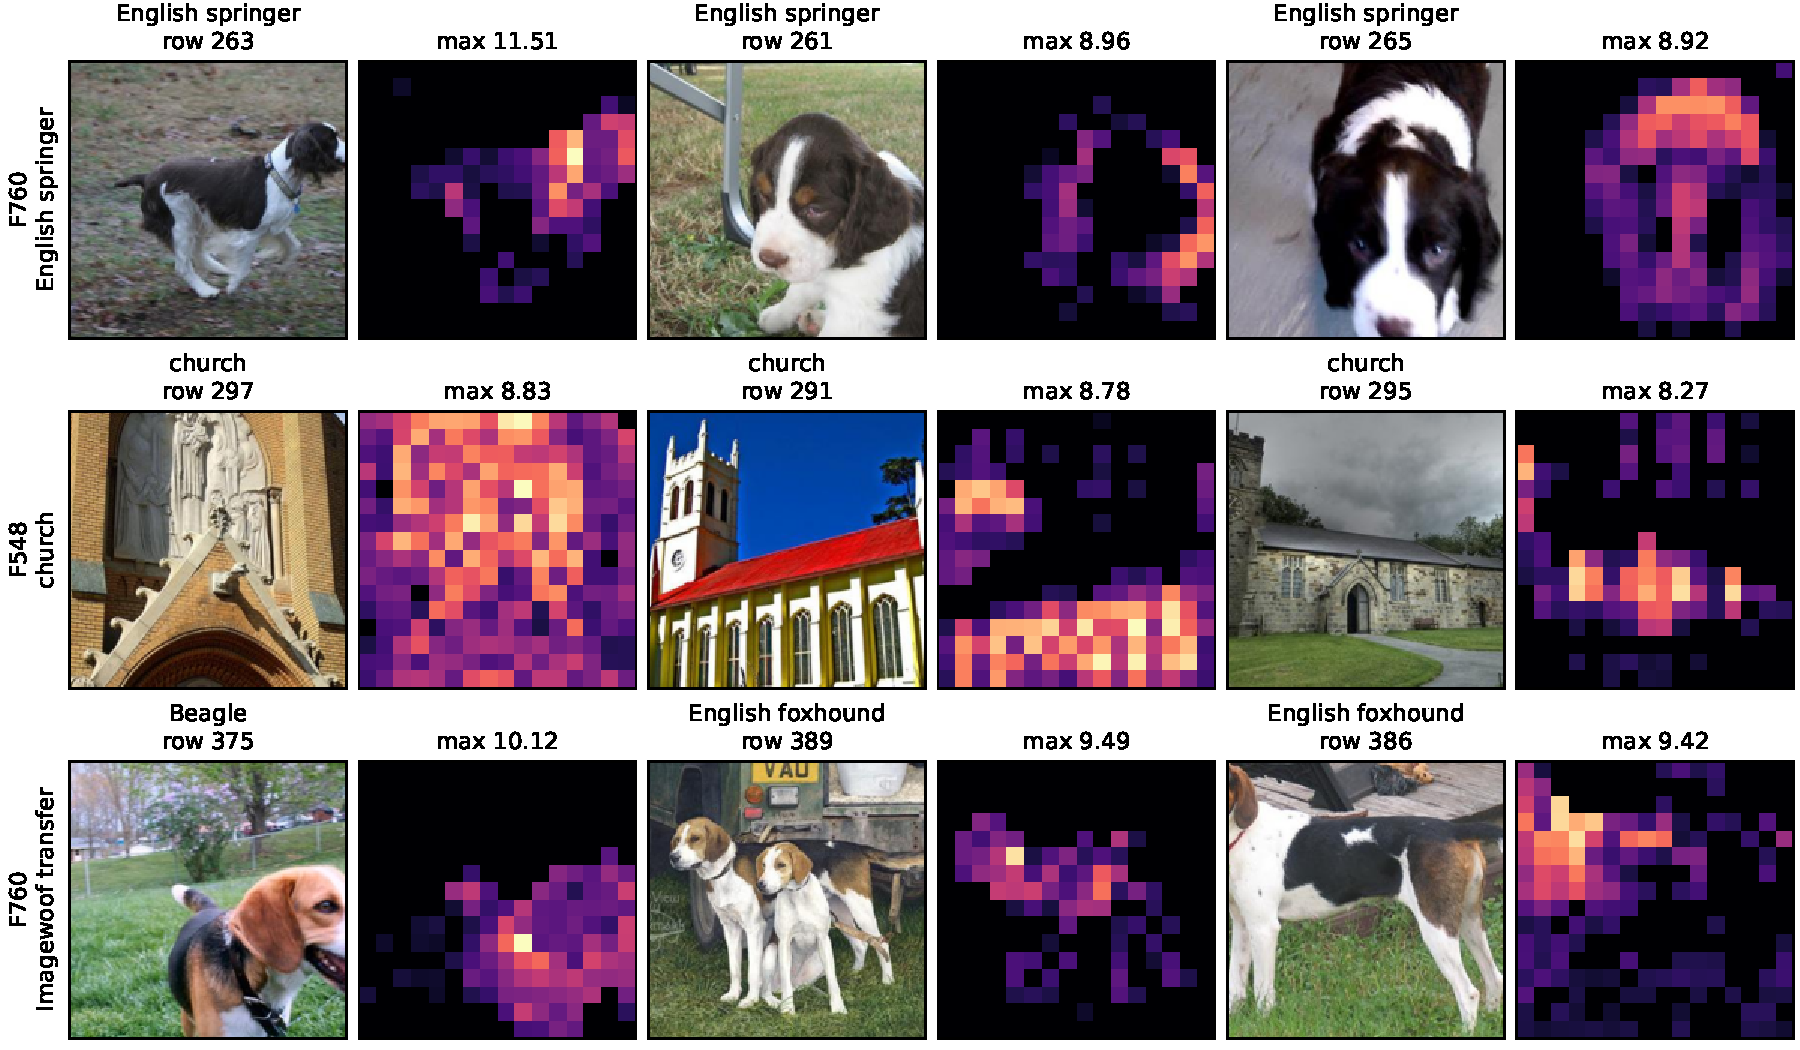
\includegraphics[width=\linewidth]{figures/imagenette_dinov2_codexgen.pdf}
    \caption{The same selection and evaluation protocol for DINOv2.
        Maps locate patch-token responses after global self-attention; they
        are not object masks. Imagenette and Imagewoof labels identify the
        photographs rather than certify the coordinate's semantic meaning.}
    \label{fig:imagenette-dino}
\end{figure}

To investigate what increases a selected response, optimize the input
pixels through the frozen backbone and SAE encoder. Let $a_{p,j}(x)$
be the encoder's affine response for coordinate $j$ at site $p$, before
ReLU and Top-$k$ gating. Define a smooth spatial objective by
\begin{equation}\label{eq:visualization-objective}
    L_{j}(x)=\frac{1}{r_{j}}
    \log\left(\frac{1}{|P|}\sum_{p\in P}\exp(a_{p,j}(x))\right)
    -0.1\operatorname{TV}_{2}(x),
\end{equation}
where $r_{j}$ is the training-image RMS of the max-pooled sparse
coordinate, floored at $10^{-6}$. Here $\operatorname{TV}_{2}$ is the
sum of mean squared horizontal and vertical adjacent-pixel differences.
The pre-gating objective avoids a zero gradient when a coordinate is
absent from the initial Top-$k$ support. It is explicitly a smooth
proxy: every resulting stimulus is also evaluated with the actual
ReLU and Top-$k$ code, which is the quantity used by the lattice queries.

Parameterize the image by a real inverse Fourier transform followed by
a sigmoid. Multiply Fourier coefficients by a radial frequency weight
proportional to $\max(\|\omega\|,1/224)^{-1.5}$, normalized to unit RMS.
Use two random initializations per coordinate, with random seed 2028,
and 120 Adam updates at learning rate 0.05. During optimization, reflect
pad by eight pixels and sample a translated $224\times224$ window.
This supplies a simple smoothness and translation prior inspired by
feature-visualization methods~\cite{olah2017featureVis}; it is not a
pixel-for-pixel implementation of Distill's parameterization. Both
initializations are retained without choosing a visually favorable one.

\begin{figure}[p]
    \centering
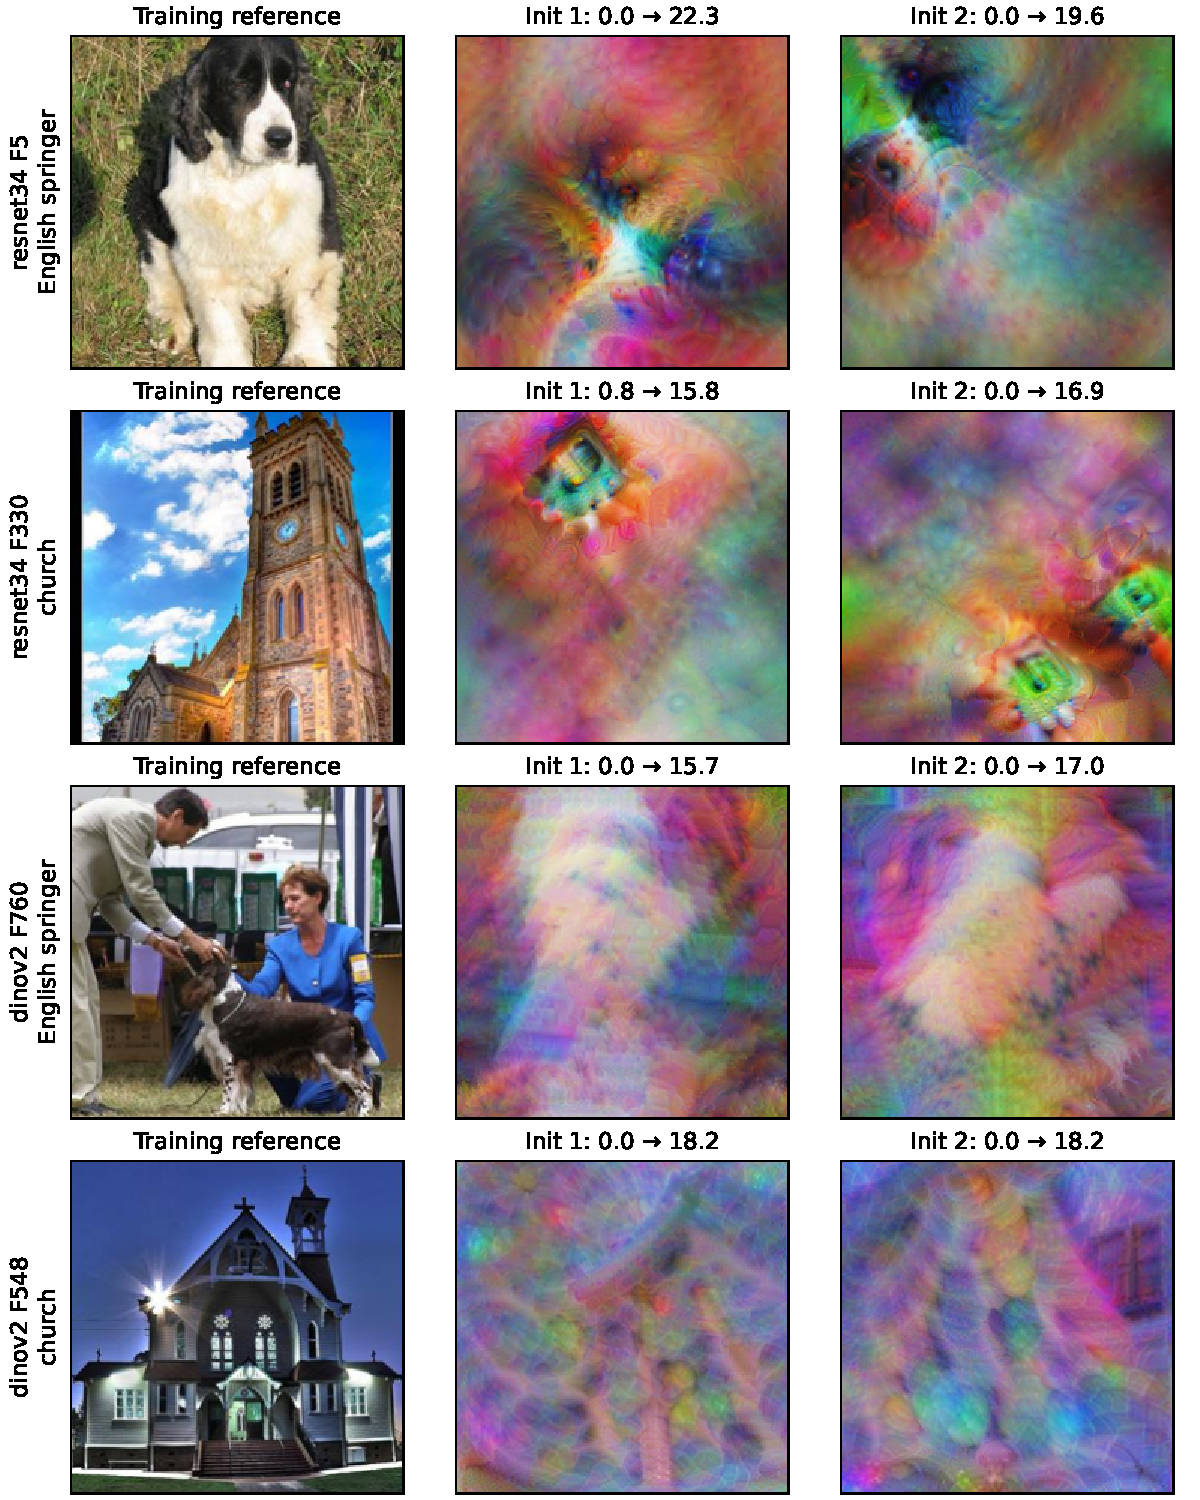
\includegraphics[width=0.9\linewidth]{figures/optimized_features_codexgen.pdf}
    \caption{Training reference photographs and two optimized stimuli per
        coordinate. Titles report actual max-pooled sparse codes before and
        after optimization, evaluated without jitter. The photographs
        initialize
        neither run: optimization starts from random Fourier parameters.
        Textures or shapes in these images suggest hypotheses, but cannot alone
        identify semantic feature meanings or a downstream computation.}
    \label{fig:optimized-features}
\end{figure}

\begin{table}[tbp]
\centering
\begin{tabular}{llrrr}
\toprule
Model & Selection & Coordinate & Test AP & Optimized codes \\
\midrule
ResNet34 & English springer & 5 & 0.748 & 22.3, 19.6 \\
ResNet34 & church & 330 & 0.458 & 15.8, 16.9 \\
DINOv2 & English springer & 760 & 1.000 & 15.7, 17.0 \\
DINOv2 & church & 548 & 0.983 & 18.2, 18.2 \\
\bottomrule
\end{tabular}
\caption{Training-selected coordinates, descriptive Imagenette test AP, and
actual optimized-stimulus codes for both fixed initializations. Class
prevalence is 0.1.}
\label{tab:imagenette-features}
\end{table}

The DINOv2 coordinates attain descriptive test AP values of 1.000 and
0.983, compared with 0.748 and 0.458 for ResNet. Each value uses only ten
positive and 90 negative Imagenette test photographs. These observations
are not uncertainty-qualified population comparisons. All eight optimized
stimuli increase the actual gated coordinate relative to their initial
images. Several optimizations nevertheless produce textures or repeated
fragments rather than a unique object, so visual resemblance needs further
testing against alternatives.

The released floating-point stimuli, initial images, optimization losses,
and measured codes permit direct verification of the displayed effects.
An increase under the smooth objective need not increase the gated code;
reporting the latter prevents that distinction from being hidden.

\subsection{Controlled probes and lattice queries}
\label{sub:feature-probes}
We next test the same coordinates on semicircular arcs, straight lines,
and right-angle corners at twelve orientations spaced by 30 degrees.
Render each shape with antialiasing, subtract its spatial mean, and
normalize its pixel standard deviation. Apply one shared contrast factor
so that all images remain in $[0,1]$ around mean gray $0.5$. Thus mean
brightness and RMS contrast are matched across the 36 stimuli. Shape
length, occupied area, and topology remain different; these probes do
not isolate curvature as the only varying factor.

\begin{figure}[tbp]
    \centering
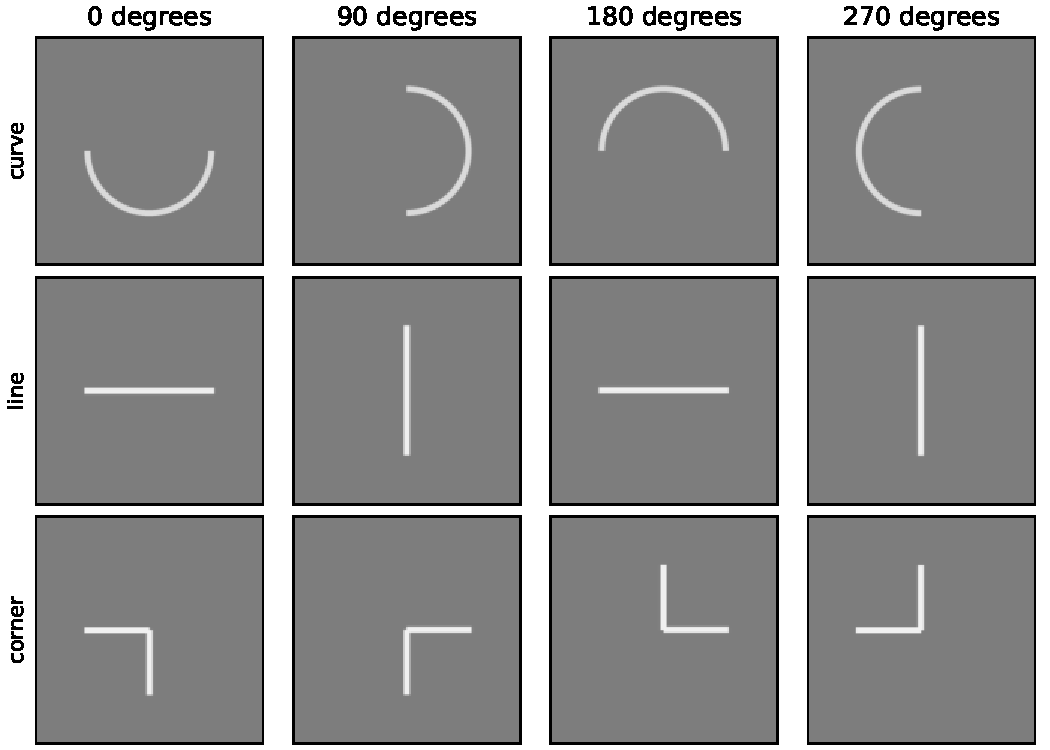
\includegraphics[width=0.7\linewidth]{figures/synthetic_stimuli_codexgen.pdf}
    \caption{Examples from the exact controlled stimulus family, shown
        at four orientations. Curves, lines, and corners have matched mean
        brightness and RMS contrast. All twelve orientations and their pixel
        arrays are retained in the evidence bundle.}
    \label{fig:synthetic-stimuli}
\end{figure}

\begin{figure}[p]
    \centering
    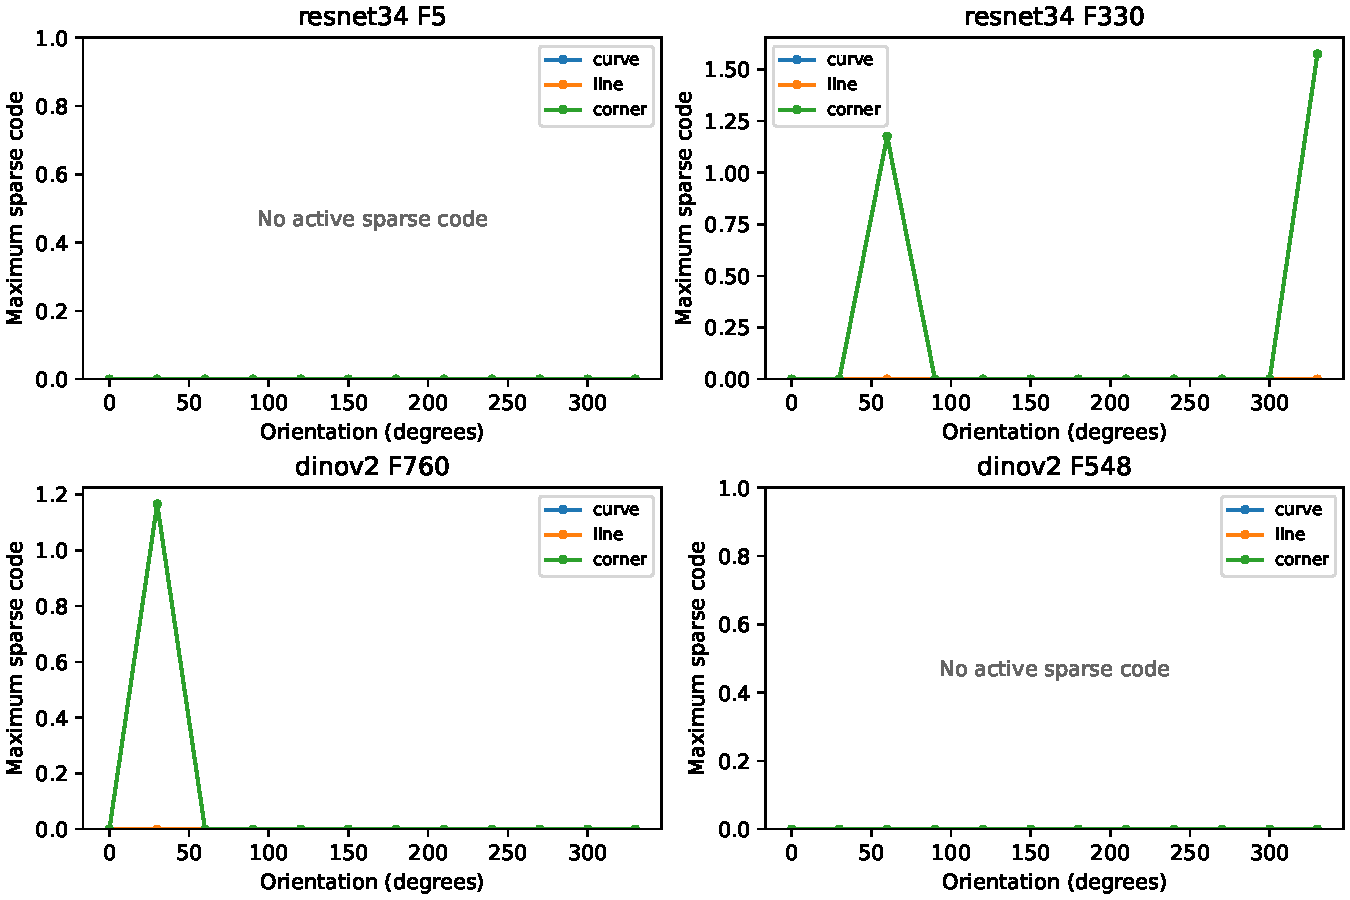
\includegraphics[width=\linewidth]{figures/synthetic_tuning_codexgen.pdf}
    \caption{Actual sparse-coordinate responses to the controlled stimuli.
        Each panel reports one training-selected coordinate. A peak or a weak
        response here is an observation on this probe family, not a
        demonstration
        that the coordinate is a curve detector. Flat zero curves mean that
        Top-$k$ gating suppresses that coordinate on these inputs.}
    \label{fig:synthetic-tuning}
\end{figure}

None of the four selected coordinates has a nonzero sparse code on the
curve or straight-line probes at these orientations. ResNet's
church-selected coordinate responds to corners at two orientations;
DINOv2's springer-selected coordinate responds to one corner orientation.
These isolated responses do not support calling any of these coordinates
a curve detector. They illustrate why a class-associated gallery and an
optimized texture are insufficient to infer elementary shape selectivity.

Separately, rotate each coordinate's strongest class-matching training
photograph by the same twelve angles. Use bilinear interpolation and gray
fill without expanding the crop. This changes orientation, but also
introduces cropping and interpolation effects; the curves in
\cref{fig:rotation-tuning} measure the combined transformation. They are
not a pose-invariance test across independent three-dimensional views.

\begin{figure}[tbp]
    \centering
    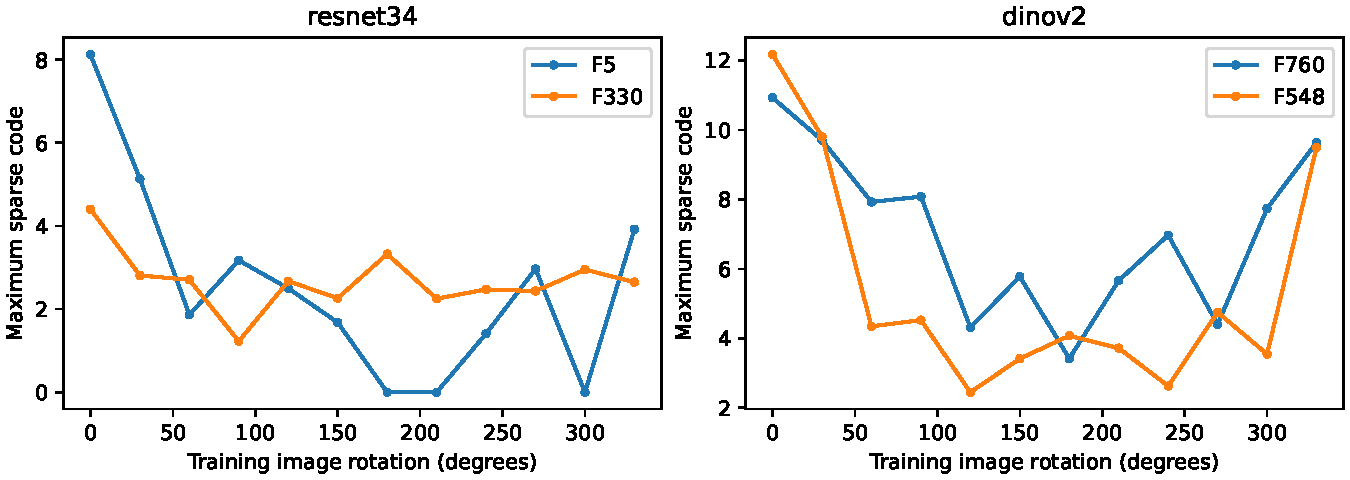
\includegraphics[width=\linewidth]{figures/rotation_tuning_codexgen.pdf}
    \caption{Responses under rotation of the fixed training references.
        Absolute code magnitudes are shown without rescaling each curve to its
        own maximum. Coordinates and backbones have different native units;
        compare transformations within a curve rather than absolute values
        across models.}
    \label{fig:rotation-tuning}
\end{figure}

Finally, construct two source queries from the selected training
photographs, retaining half their activation on the two selected
coordinates and setting all other coordinates to zero. Compute their
meet and join exactly as in~\cref{sub:natural-queries}. Evaluate on the
200-image union of Imagenette test and Imagewoof transfer images.
\begin{table}[tbp]
    \centering
    \begin{tabular}{llrr}
        \toprule
        Model    & Query & Pooled matches & Same-site matches \\
        \midrule
        ResNet34 & u     & 11             & 1                 \\
        ResNet34 & v     & 14             & 14                \\
        ResNet34 & meet  & 61             & 61                \\
        ResNet34 & join  & 5              & 1                 \\
        DINOv2   & u     & 26             & 3                 \\
        DINOv2   & v     & 8              & 8                 \\
        DINOv2   & meet  & 86             & 86                \\
        DINOv2   & join  & 0              & 0                 \\
        \bottomrule
    \end{tabular}
    \caption{Query extents on the 200 evaluation photographs. The meet and join
        combine source activation requirements.}
    \label{tab:imagenette-queries}
\end{table}

ResNet's join retrieves five images but has only one same-site witness;
DINOv2's join is empty. These are different learned queries, so the counts
are not a retrieval-quality ranking of the backbones.
The join extent is the intersection of the two source extents, whereas
same-site counts impose an additional common-witness condition. These
are operations on numerical evidence, not claims that an image belongs
to both selection classes. The transformer example retains exactly the
same order-theoretic semantics despite its globally contextualized tokens.


\subsection{Meet and join galleries on Imagenette}
\label{sub:imagenette-query-galleries}
To see the operations on recognizable photographs, we now compare
queries within the English springer and garbage truck classes. These
are additional queries, distinct from the springer/church pair in
\cref{tab:imagenette-queries}. For each class and backbone, rank
coordinates by training contrast as in~\cref{eq:feature-contrast} and
keep the first two. Select a class-matching training photograph with
maximal activation of the first coordinate, then a distinct photograph
with maximal activation of the second coordinate. Break coordinate ties
by index and photograph ties by stored row. The distinctness restriction
ensures two source photographs even if both coordinates peak on the
same training image. No held-out photograph chooses a coordinate,
source, or threshold.

As before, retain half of both source-image coordinate values, setting
all other coordinates to zero. Compute the meet by coordinatewise
minimum and the join by coordinatewise maximum. Evaluate on all 100
Imagenette test photographs; Imagewoof is excluded from these galleries.
Each row displays up to three satisfying photographs ranked by
\cref{eq:graded-score}, with ties broken by stored row. Counts cover
all 100 photographs, not just the displayed examples. Titles give
actual labels and dataset rows; the released arrays map these rows to
original archive paths. Thresholds and scores in the figures are rounded
only for display. A \emph{site: yes} annotation means that some single
site meets every positive threshold; it is not a segmentation or causal
localization claim.

\Cref{fig:imagenette-springer-resnet,fig:imagenette-springer-dino}
compare the springer-selected coordinates. ResNet's source extents have
sizes 5 and 3, the meet has size 6, and the join has size 2. Every
same-site extent is empty: the positive requirements are met at
separate spatial witnesses. DINOv2 retrieves the same ten photographs
for all four pooled queries, although thresholds and rankings differ.
Its same-site counts are 6, 6, 7, and 5. Thus identical pooled extents
can conceal differences in both graded satisfaction and common-site
evidence. This observation concerns two independently learned queries;
it does not establish superior spatial localization by a transformer.

\begin{figure}[p]
    \centering
    \includegraphics[width=\linewidth]{%
        figures/query_springer_resnet34_codexgen.pdf}
    \caption{Imagenette springer queries for ResNet34 on coordinates
        $(5,357)$. The top row shows the training sources. Subsequent rows
        show source queries, their meet, and their join, followed by ranked
        test matches. Here $s$ is the graded satisfaction ratio. The join
        has two matches; the third position is explicitly empty. None of
        the pooled matches has a common-site witness.}
    \label{fig:imagenette-springer-resnet}
\end{figure}

\begin{figure}[p]
    \centering
    \includegraphics[width=\linewidth]{%
        figures/query_springer_dinov2_codexgen.pdf}
    \caption{The same within-class selection protocol for DINOv2,
        on coordinates $(760,556)$. All four pooled extents contain the
        same ten test photographs, while rankings and same-site counts
        change. Only the three highest-ranked matches per row are shown.
        Transformer sites denote globally contextualized patch tokens.}
    \label{fig:imagenette-springer-dino}
\end{figure}

The truck examples in
\cref{fig:imagenette-truck-resnet,fig:imagenette-truck-dino} also show
why a meet extent need not equal the union of the source extents.
ResNet's source extents have sizes 9 and 8, their join has size 8,
and their meet has size 10. One photograph therefore satisfies the
meet but neither source query: relaxing different coordinates can admit
an additional combination of evidence. The corresponding same-site
counts are 1, 0, 1, and 0. DINOv2 again has ten pooled matches for every
operation, with same-site counts 10, 10, 10, and 9. Across these four
examples, the join extent is exactly the intersection of the two source
extents, as the order-theoretic construction requires.

\begin{figure}[p]
    \centering
    \includegraphics[width=\linewidth]{%
        figures/query_truck_resnet34_codexgen.pdf}
    \caption{Imagenette garbage-truck queries for ResNet34 on
        coordinates $(100,302)$. The meet retrieves ten photographs,
        including one outside the union of the source extents. The top
        right inset shows this extra photograph with its satisfaction
        ratios for the two sources and their meet. The join
        retains eight pooled matches but no common-site witness. Labels
        describe photographs rather than meanings assigned to coordinates.}
    \label{fig:imagenette-truck-resnet}
\end{figure}

\begin{figure}[p]
    \centering
    \includegraphics[width=\linewidth]{%
        figures/query_truck_dinov2_codexgen.pdf}
    \caption{Imagenette garbage-truck queries for DINOv2 on
        coordinates $(714,205)$. All ten pooled matches survive the join,
        but one loses a common-site witness. This difference uses all
        test matches, including those outside the three displayed ranks.}
    \label{fig:imagenette-truck-dino}
\end{figure}

These examples make threshold combination and spatial witnessing
inspectable at photographic resolution. The two features in each pair
were selected by the same class contrast; we have not identified them
as distinct parts, colors, or shapes. Neither a coherent gallery nor
an unchanged extent proves that two coordinates have the same meaning.
The saved source values, query vectors, full rankings, and site masks
allow these numerical observations to be checked independently.

Taken together, the photographs, optimized stimuli, and controlled
responses provide a more demanding feature investigation than a gallery
alone. Recovering a circuit would require additional evidence about how
upstream features construct the response and how downstream computations
use it, as distinguished in~\cite{olah2020zoom}. No such circuit recovery
is claimed by these experiments.
